\documentclass{beamer}

\usepackage[utf8]{inputenc}
\usepackage{tikz}
\usepackage{gnuplottex} % [noshell]: do not regenerate gnuplots

\usepackage{booktabs}
\usepackage{listings}
\lstset{
  language=python,
  basicstyle=\scriptsize,
}
\usetheme{ODK}

\AtBeginSection[]
{
  \begin{frame}<beamer>
    \frametitle{Outline}
    \tableofcontents[currentsection]
  \end{frame}
}

\title[Workpackage 5]{Workpackage 5:\\ High Performance Mathematical Computing}

\author[2nd projet review]{Clément Pernet}

\date{Luxembourg, October 30, 2018}

\institute[ODK Project review]{Second OpenDreamKit Project review}

\begin{document}
\maketitle

%%%%%%%%%%%%%%%%%%%%%%%%%%%%%%%%%%%%%%%
\section*{Introduction}

\begin{frame}
  \frametitle{High performance mathematical computing}

  \begin{block}{Computer algebra}
    Typical computation domains:
    \begin{itemize}
    \item $\mathbb{Z}, \mathbb{Q}$: $\leadsto$ multiprecision integers
    \item $\mathbb{Z}/p\mathbb{Z}, \mathbb{F}_q$: $\leadsto$ machine ints or
      floating point, multiprecision
    \item $K[X], K^{m\times n}$, $K[X]^{m\times n}$ for $K=\mathbb{Z},\mathbb{Q},\mathbb{Z}/p\mathbb{Z}$
    \end{itemize}
  \end{block}

  \begin{block} {High performance computing}
    \begin{itemize}
    \item Decades of development for numerical computations
    \item Still at an early development stage for computer algebra
    \item Specificites: cannot blindly benefit from numerical HPC experience
    \end{itemize}
  \end{block}
\end{frame}
%%%%%%%%%%%%%%%%%%%%%%%%%%%%%%%%%%%%%%%%%%%%%%%%%%%%%%%%%%%%%%%%%
\begin{frame}
  \frametitle{Goal: delivering high performance to maths users}

\uncover<2->{
  \only<1,2>{
    \begin{block}{Harnessing modern hardware $\leadsto$ parallelisation}
  \begin{itemize}
    \item in-core parallelism (SIMD vectorisation)
    \item multi-core parallelism
    \item distributed computing: clusters, cloud
    \end{itemize}
  \end{block}
  }
  
  \only<3>{
    \begin{block}{Languages}
    \begin{itemize}
    \item Computational Maths software uses high level languages (e.g. Python)
    \item High performance delivered by languages close to the metal (C, assembly)
    \end{itemize}
    $\leadsto$ compilation,  automated optimisation
  \end{block}
  }
  }
  \begin{center}
    \only<1>{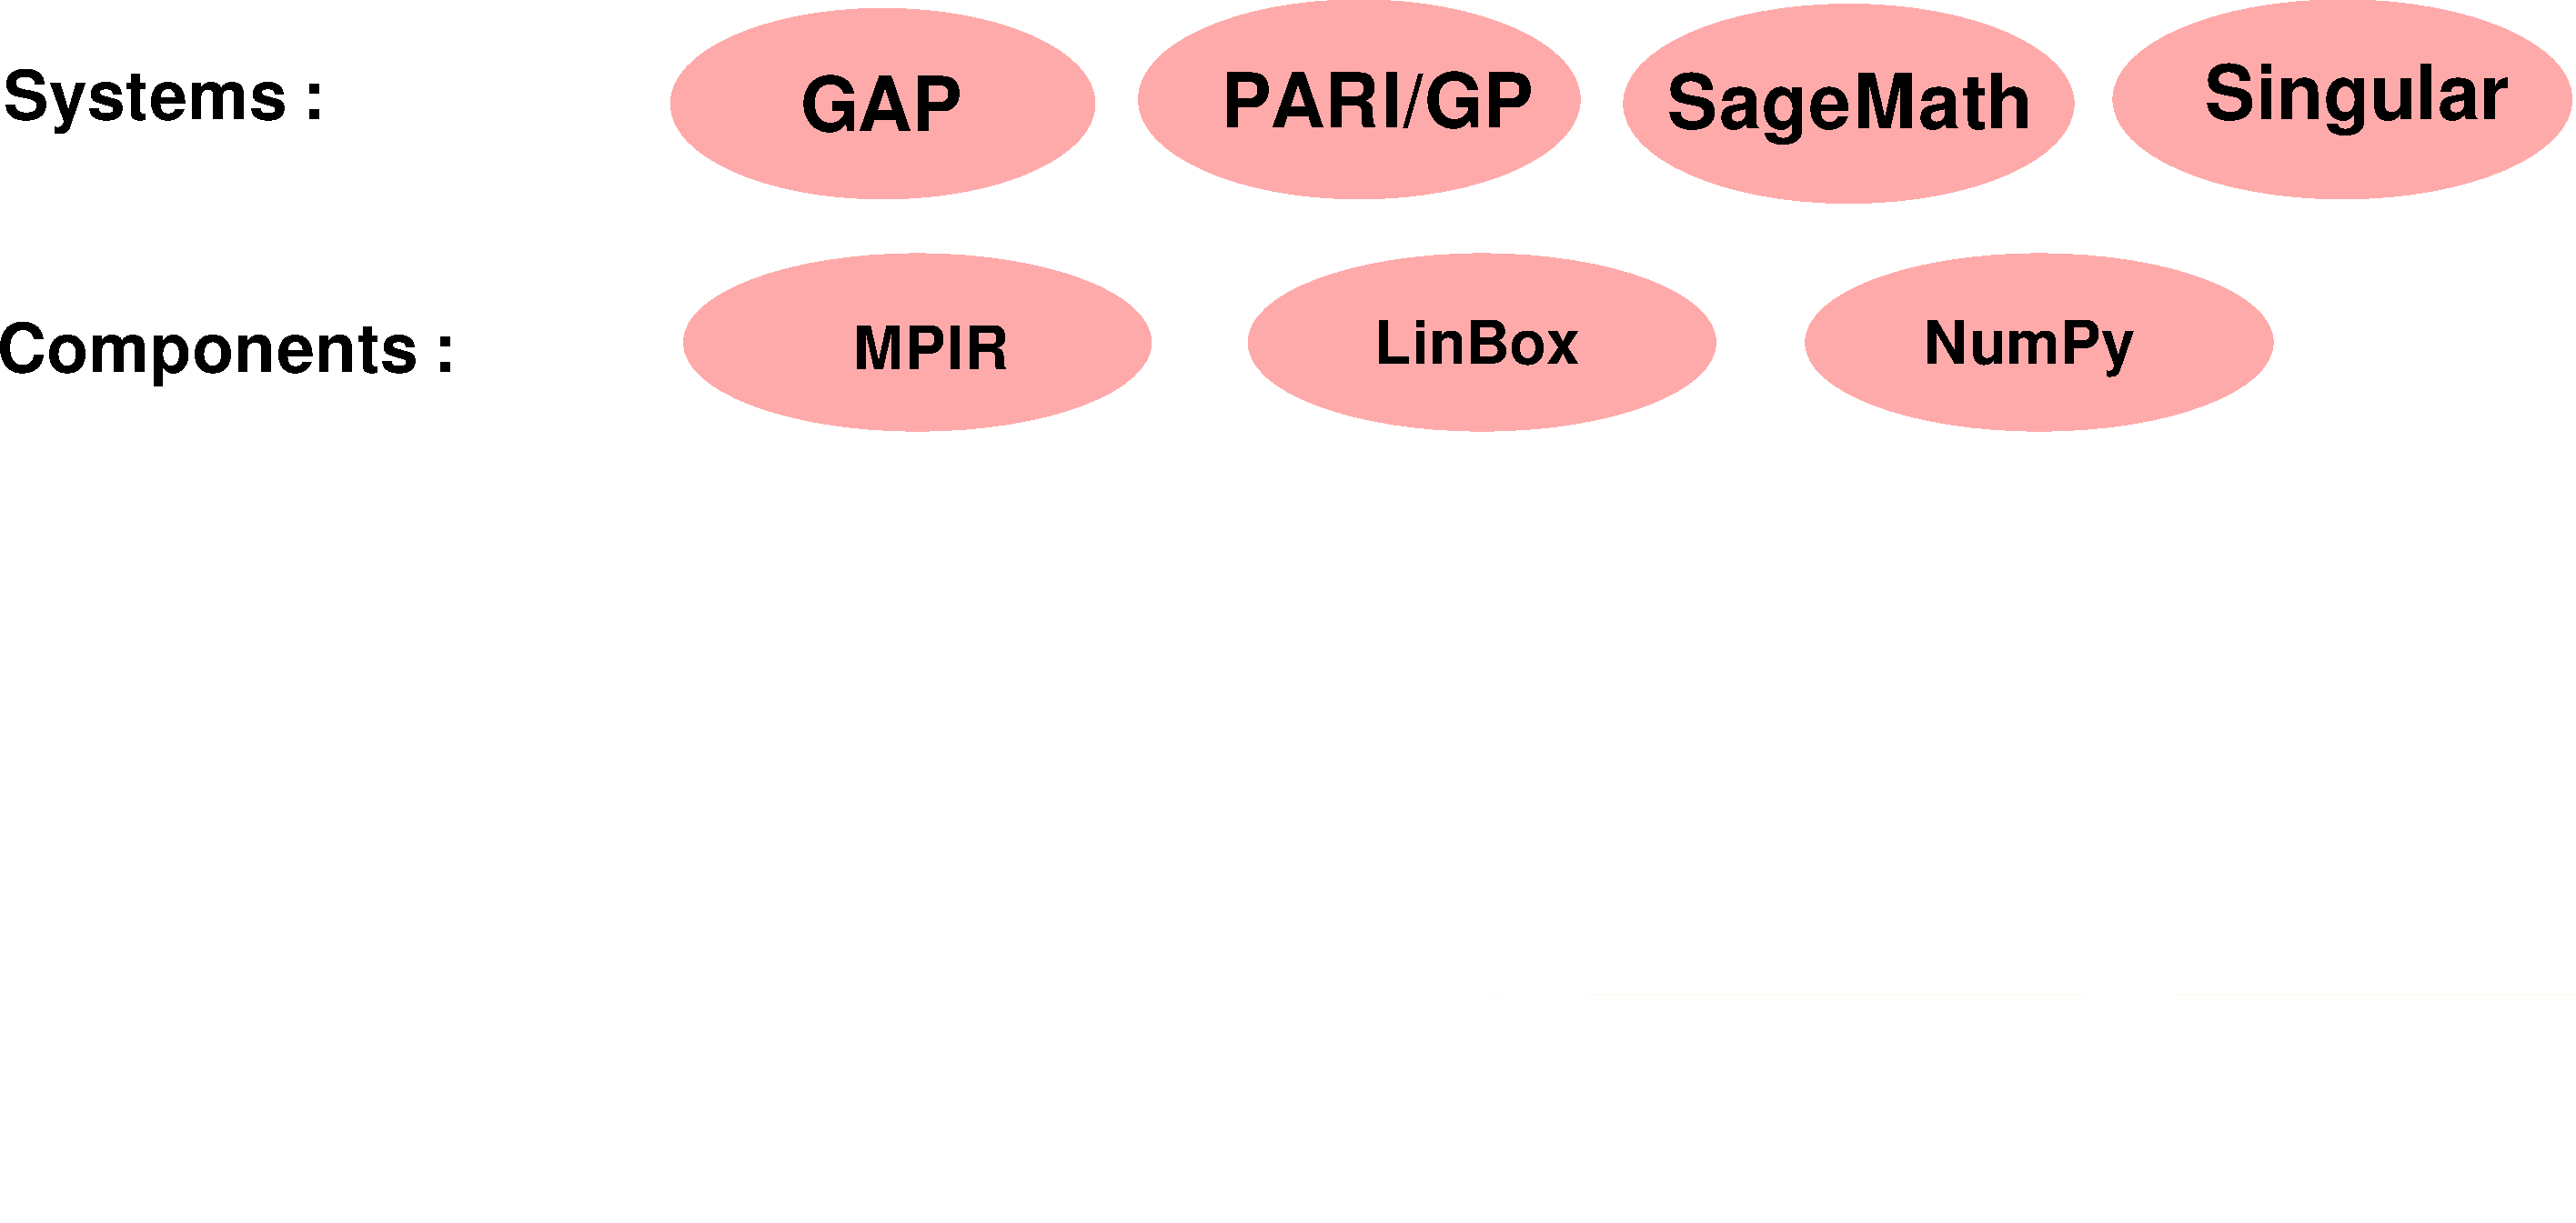
\includegraphics[width=0.8\textwidth]{software_stack_3}}

    \only<2>{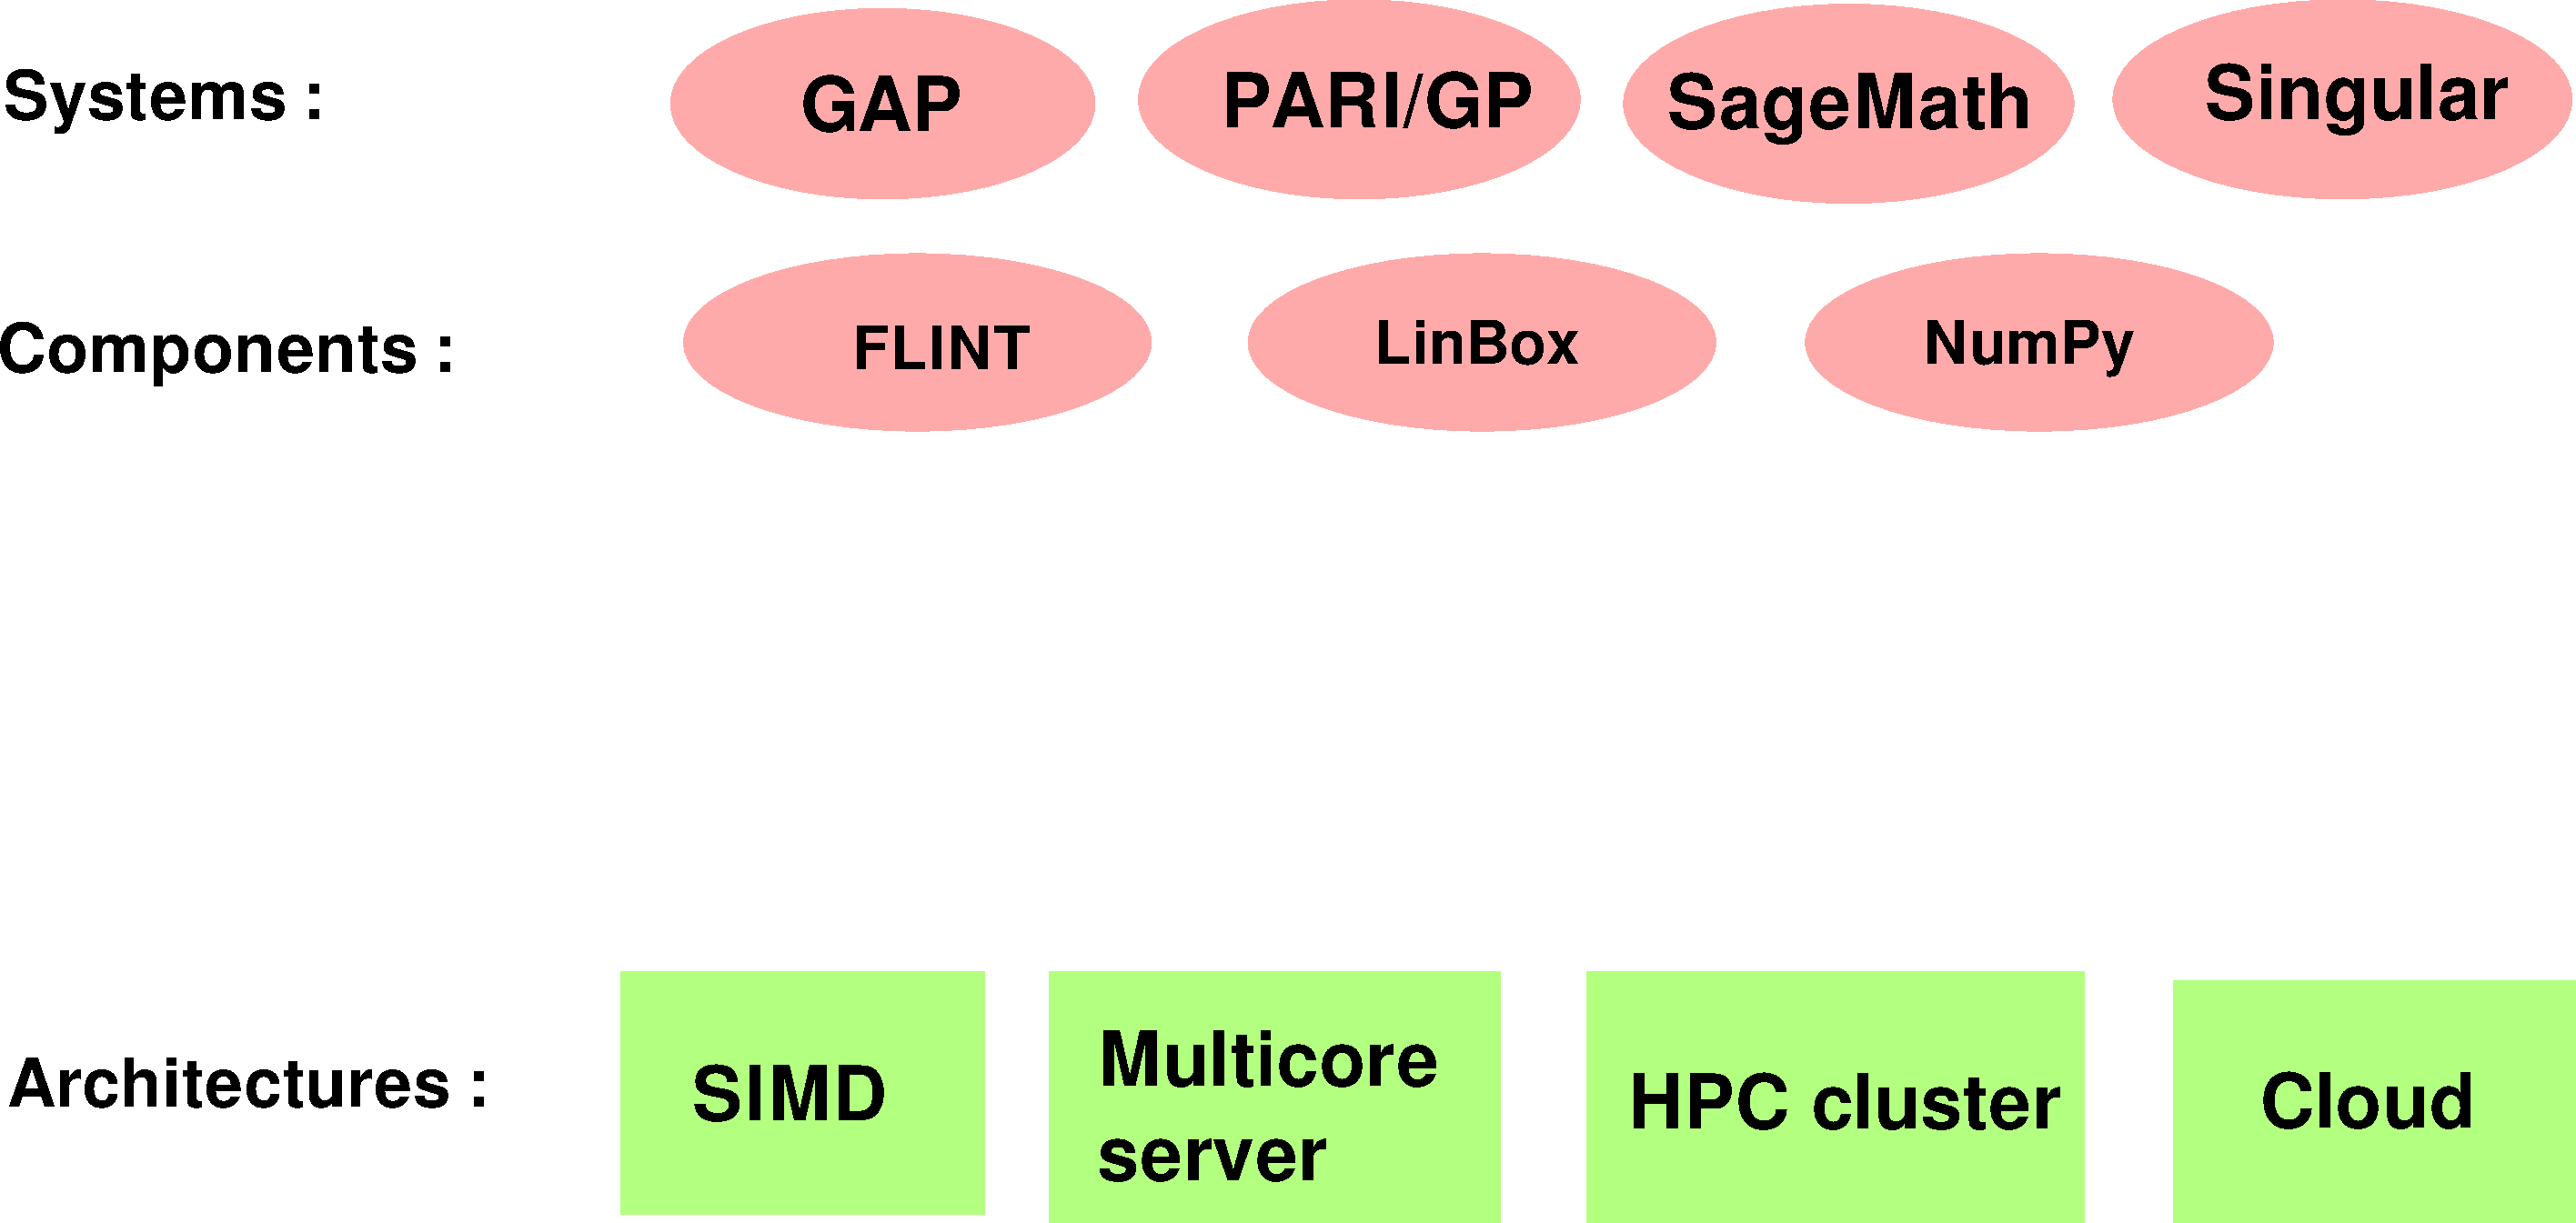
\includegraphics[width=0.8\textwidth]{software_stack_2}}
    
    \only<3>{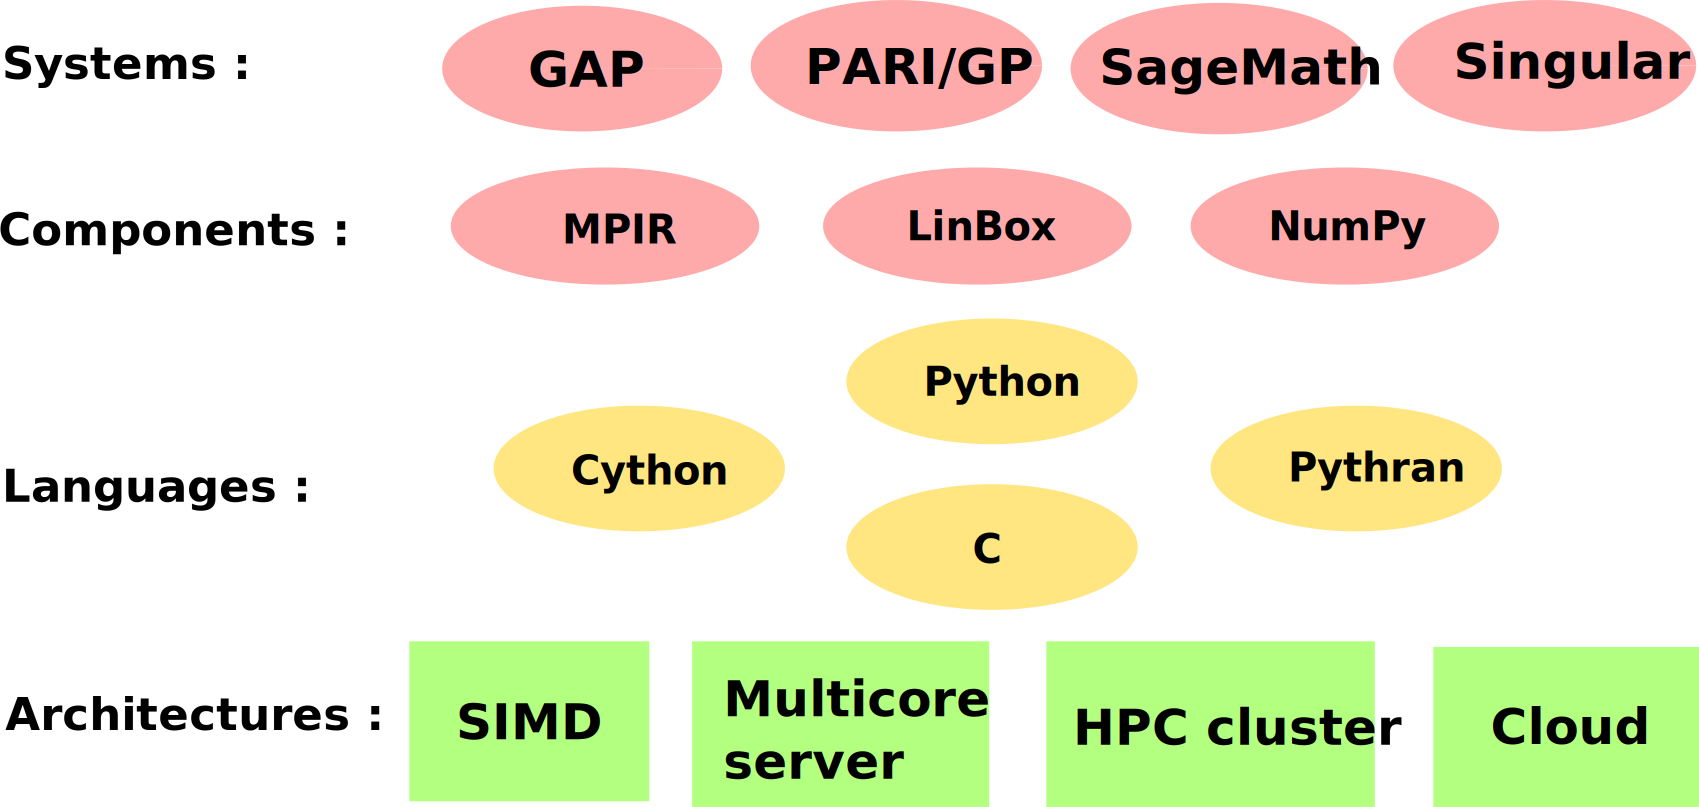
\includegraphics[width=0.8\textwidth]{software_stack}}
\end{center}

\end{frame}
%%%%%%%%%%%%%%%%%%%%%%%%%%%%%%%%%%%%%%%%%%%%%%%%%%%%%%%%%
%% \begin{frame}
%%   \frametitle{Goal: delivering high performance to maths users}

%%     \begin{center}
%%     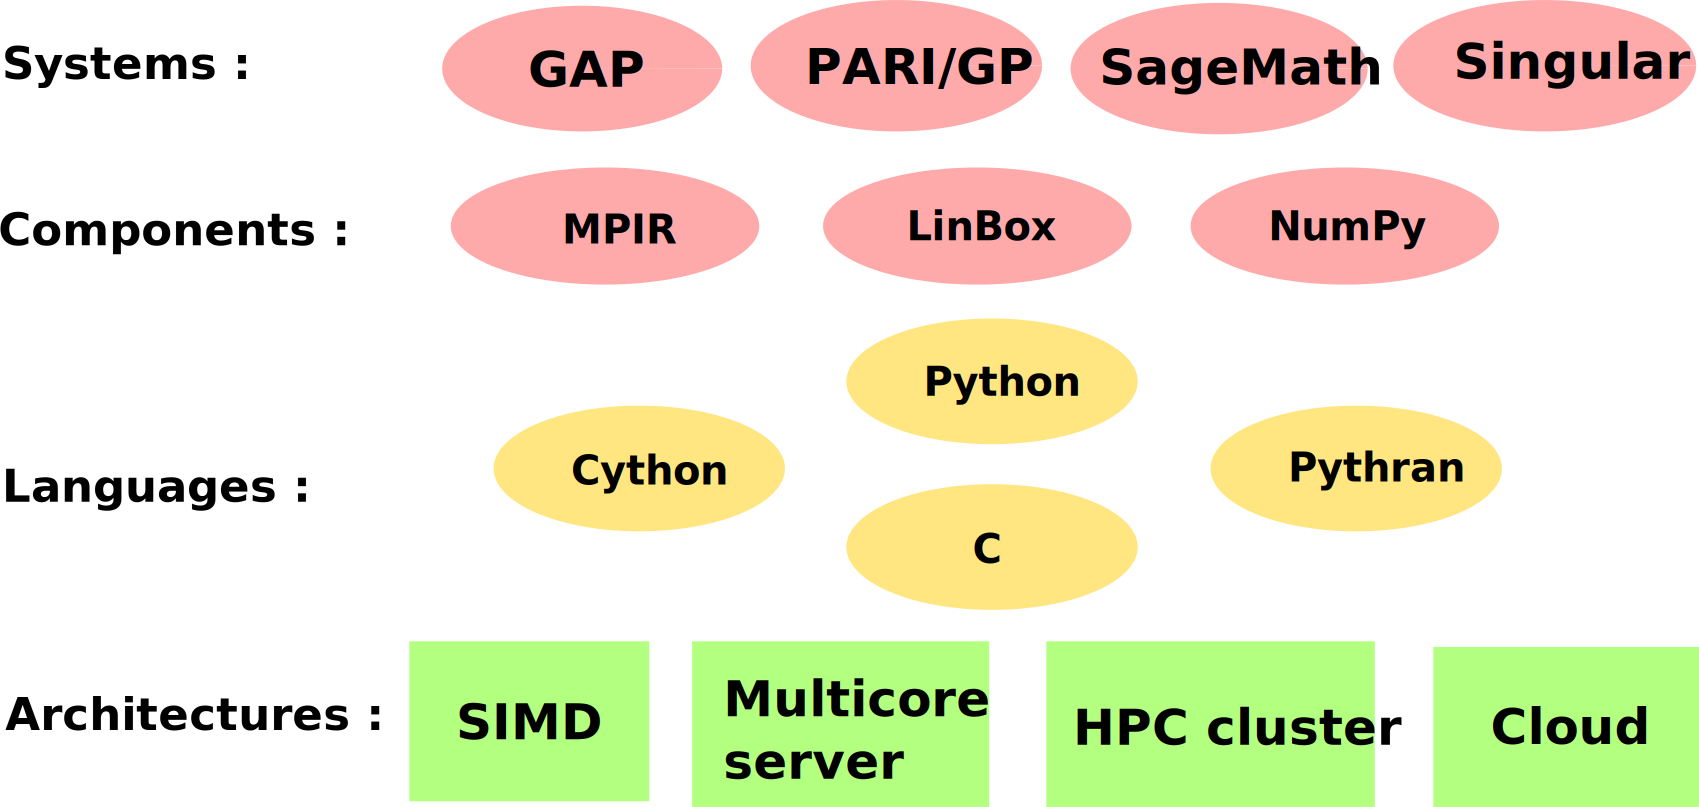
\includegraphics[width=0.8\textwidth]{software_stack}
%%   \end{center}

%%     \pause
%%     \begin{itemize}
%%     \item Improve/Develop parallel features of components first,
%%     \item Expose them through the software stack
%%     \item 
%%     \end{itemize}

%% \end{frame}


%%%%%%%%%%%%%%%%%%%%%%%%%%%%%%%%%%%%%%%
\begin{frame}
  \frametitle{Introduction}
  \begin{block}
    {Goal:}
    \begin{itemize}
    \item Offer High Performance Computing to VRE's users
    \item Improve/Develop parallel computing features of dedicated software
      kernels
    \item Expose them through the software stack
    \end{itemize}
  \end{block}
\end{frame}

%%%%%%%%%%%%%%%%%%%%%%%%%%%%%%%%%%%%%%%
\begin{frame}
  {Outline}
  \tableofcontents
\end{frame}

%%%%%%%%%%%%%%%%%%%%%%%%%%%%%%%%%%%%%%%
\section{Deliverables under review for the period}
%%%%%%%%%%%%%%%%%%%%%%%%%%%%%%%%%%%%%%%
\subsection{Task 5.3: LinBox}

\begin{frame}
  \frametitle{Task 5.3: LinBox library}
  
\end{frame}
%%%%%%%%%%%%%%%%%%%%%%%%%%%%%%%%%%%%%%%
\begin{frame}
  \frametitle{D5.12: Exact linear algebra algorithms and implementations. Library maintenance and close integration in mathematical software for LinBox library}

  \begin{enumerate}
  \item Algorithmic innovations:
    \begin{enumerate}
    \item Rank deficient dense Gaussian elimination
    \item Quasiseparabile matrices
    \item Outsourced computing security
    \end{enumerate}
  \item Software releases and integration:
    \begin{enumerate}
    \item LinBox ecosystem: \texttt{LinBox, fflas-ffpack, givaro}
    \item \texttt{SageMath} integration
    \end{enumerate}
  \end{enumerate}
\end{frame}

%%%%%%%%%%%%%%%%%%%%%%%%%%%%%%%%%%%%%%%
\begin{frame}
  \frametitle{Rank deficient dense Gaussian elimination}
  \begin{block}
    {[JSC'17] Fast computation of the rank profile matrix and the generalized
      bruhat decomposition.}
{    \small
  \begin{itemize}
    \item Connecting Rank Profile Matrix and row and column echelon forms
    \item $O\tilde\ (r^\omega + mn)$ probabilistic time
    \item generalization over arbitrary rings
    \end{itemize}
}
  \end{block}

  \begin{block}<2->{[ISSAC'18] Symmetric triangular factorization}
    \begin{columns}
      \begin{column} {.65\textwidth}
        \begin{itemize}
        \item First unconditional recursive algorithm
        \item Pivoting revealing the Rank Profile Matrix
        \item $O(n^2r^{\omega-2}) $ ($=1/3n^3$ with $\omega=3, r=n$)
        \end{itemize}
      \end{column}
      \begin{column} {.3\textwidth}
        \begin{center}
          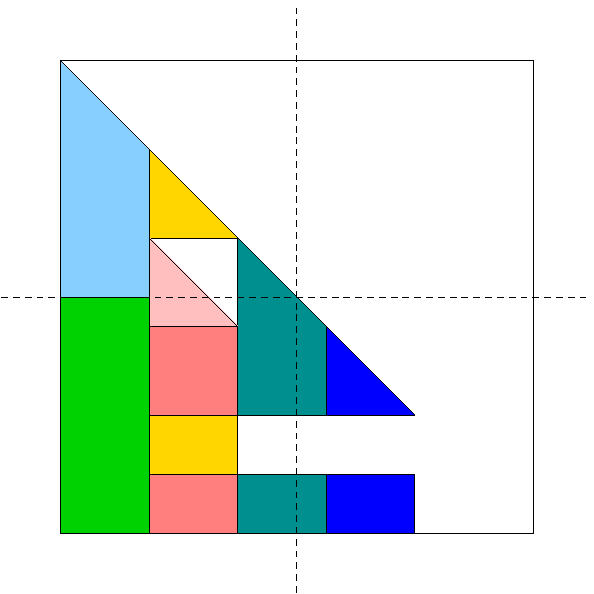
\includegraphics[width=\textwidth]{ARrec11}
        \end{center}
      \end{column}
    \end{columns}
  \end{block}
\end{frame}

%%%%%%%%%%%%%%%%%%%%%%%%%%%%%%%%%%%%%%%%%%%%%%%%%%%%%%%%%%%%%%%  
\begin{frame}[fragile]
\frametitle{LAPACK vs FFPACK modulo $8\,388\,593$}

{\footnotesize
  \begin{center}
\begin{tabular}{rrrrr}
\toprule
& \multicolumn{2}{c}{LAPACK}&\multicolumn{2}{c}{FFPACK}\\
$n$ & dgetrf (LU)  & dsytrf (LDLT) & fgetrf (LU)& fsytrf (LDLT)\\
\midrule
5000 &  2.01s & 1.60s  & 3.90s& \alert{1.59s} \\
10000 &  14.95s & 11.98s  & 24.12s& \alert{10.90s} \\
\bottomrule
\end{tabular}
\end{center}
}
%\vspace{-5pt}
%\hspace{-20pt}
%\begin{minipage}{\textwidth}
\scriptsize
%\onslide+<2>
\begin{center}
  \begin{gnuplot}[terminal=cairolatex,terminaloptions={font ",10" linewidth 2}]
  set style line 3 pt 3 pi 50 lw 4 lt rgb "blue"
  set title 'Full rank, 1-core Intel Haswell i5-4690, \symbol{64}3.5GHz' offset 0,-0.75
  set ylabel 'Effective Gfops' offset 1,0
  set xlabel 'matrix dimension' offset 0,0.1
  set xtics rotate by 30 offset -2,-0.75
  set y2tics autofreq 
  set autoscale y2fixmin
  set autoscale y2fixmax  
  set size 0.8,0.75
  set key bottom right Left reverse
  plot [1:10000] [1:45] \
  "data_gflops.txt" using 1:2 title "LAPACK dgetrf" with lines lw 4 lc 1, \ 
  "data_gflops.txt" using 1:3 title "LAPACK dsytrf" with lines lw 4 lc 2, \
  "data_gflops.txt" using 1:6 title "FFPACK fgetrf" with lines lw 4 lc 4, \
  "data_gflops.txt" using 1:7 title "FFPACK fsytrf" with lines ls 3
\end{gnuplot}
\end{center}
%\end{minipage}
\end{frame}
%%%%%%%%%%%%%%%%%%%%%%%%%%%%%%%%%%%%%%%
\begin{frame}
  \frametitle{Quasiseparable matrices }
  \begin{center}
    \textit{Matrices with low off-diagonal rank}
  \end{center}

  \begin{block}
    {[ISSAC'16, JSC'18] New compact representation and algorithms}
  \begin{columns}
    \begin{column}{.6\textwidth}
    \begin{itemize}
    \item Connection with rank profile matrix
    \item Matches the best space complexities: $O(ns)$
    \item Reduction to matrix multiplication: $O(ns^{\omega-1})$ for products
    \item Flat representation (non hierarchical)
    \end{itemize}
    \uncover<2->{
      \begin{description}
      \item[Follow-up:] on-going collaboration with numerical HPC experts:
        \begin{itemize}
        \item S. Chandrasekaran (UCal)
        \item T. Mary (U. Manchester, \texttt{Mumps})
        \end{itemize}
      \end{description}
      }
    \end{column}
    \begin{column}{.3\textwidth}
      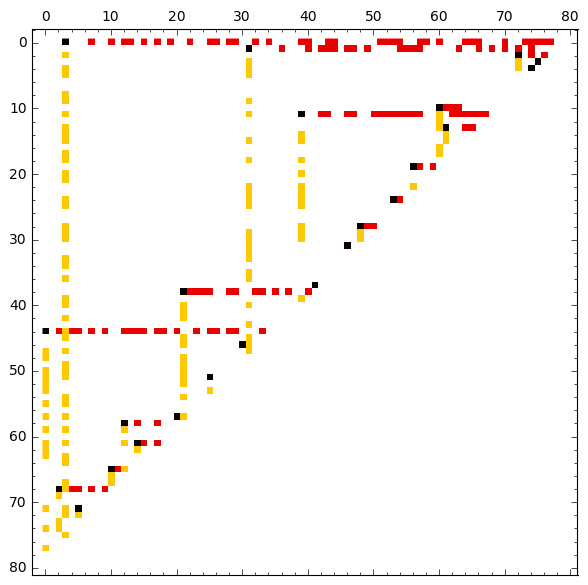
\includegraphics[width=\textwidth]{Bruhat}
    \end{column}
  \end{columns}
  \end{block}

\end{frame}


%%%%%%%%%%%%%%%%%%%%%%%%%%%%%%%%%%%%%%%
\begin{frame}
  \frametitle{Outsourced computing security}

  Exploratory 
\end{frame}
%%%%%%%%%%%%%%%%%%%%%%%%%%%%%%%%%%%%%%%
%%%%%%%%%%%%%%%%%%%%%%%%%%%%%%%%%%%%%%%
\subsection{Task 5.6: Combinatorics}
\begin{frame}
  \frametitle{Task 5.6: HPC infrastructure for Combinatorics}

  \begin{center}
    {\bf \large
      Perform a Map/Reduce on huge {\color{blue} recursive} datasets.
      }
  \end{center}

  \begin{block}{Large range of intensive applications in combinatorics}
    \begin{itemize}
    \item Test a conjecture: i.e. find an element of $S$ satisfying a certain
      property
    \item Count/list the elements of $S$ having this property
    \end{itemize}
  \end{block}

  \begin{block}{Specificities of combinatorics}
    \begin{itemize}
    \item Sets  often \textit{don't fit in the computer's memory/disk} and are
      enumerated \textbf{on the fly}: ($10^{17}$ bytes)
    \item \textbf{Embarassingly parallel}, if the set is flat (a list a file,
      stored on a disk)
    \item Recursive data-structure may be heavily unbalanced
    \end{itemize}
  \end{block}
\end{frame}
%%%%%%%%%%%%%%%%%%%%%%%%%%%%%%%%%%%%%%%
\begin{frame}
  \frametitle{D5.11: Refactor and Optimise the existing combinatorics Sage code using the new developed Pythran and Cython features.}
\end{frame}

%%%%%%%%%%%%%%%%%%%%%%%%%%%%%%%%%%%%%%%
%% \subsection{Task 5.7: Pythran}
%% \begin{frame}
%%   \frametitle{Task 5.7: Pythran}
%%   \begin{center}
%%     {\Large \textbf{Pythran}: a Python to C compiler}
%%   \end{center}
%%   \begin{columns}
%%     \begin{column}
%%       {.48\textwidth }
%%           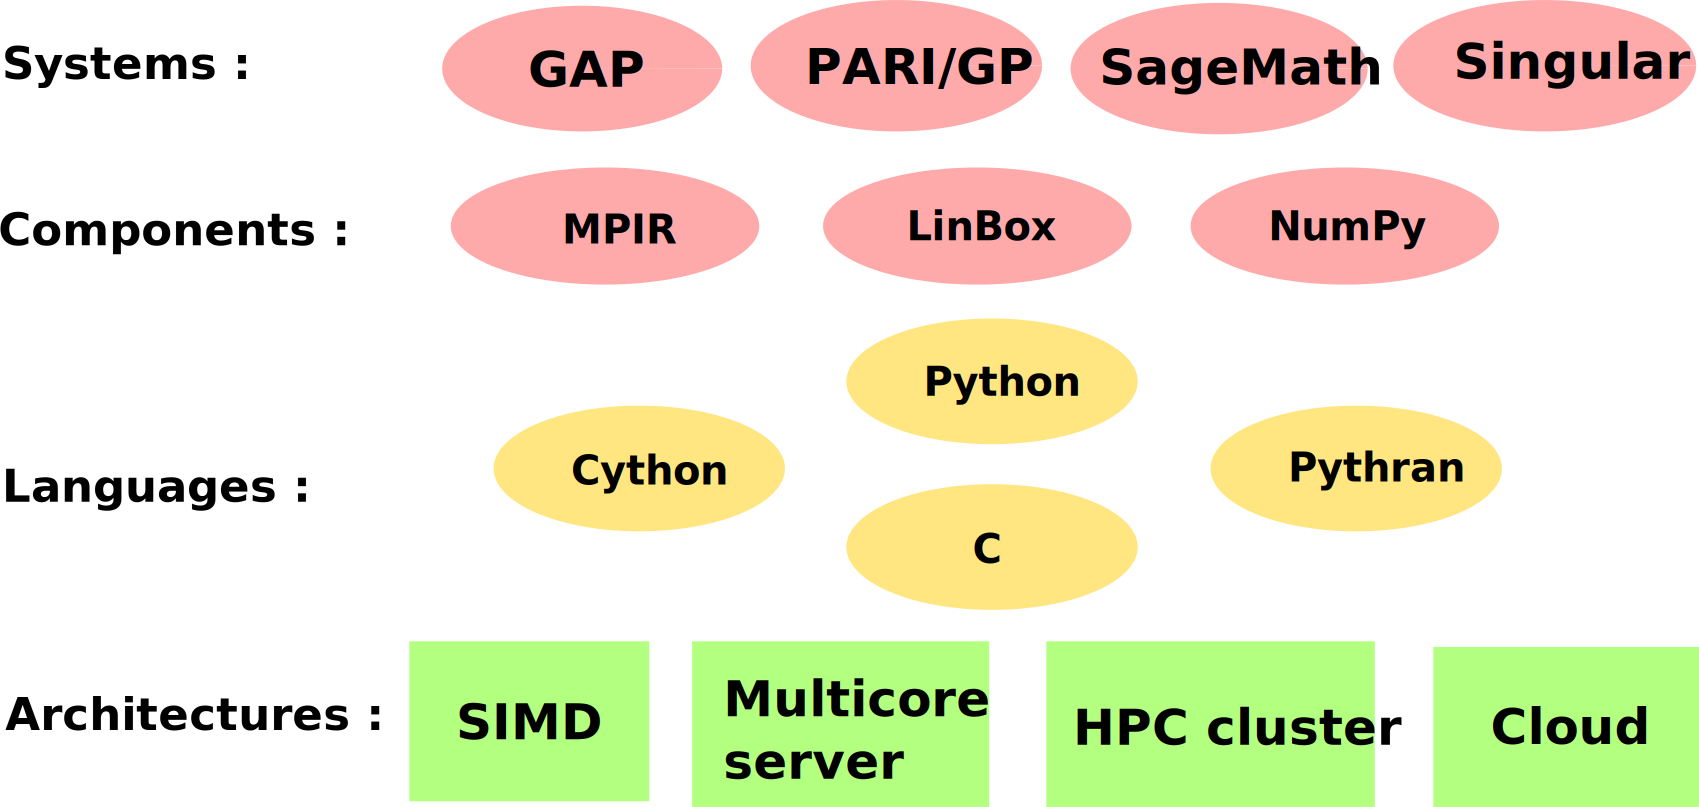
\includegraphics[width=\textwidth]{software_stack}
%%     \end{column}
%%     \begin{column}
%%       {.48\textwidth }
%%   \begin{itemize}
%%   \item High level VRE rely on the Python language
%%   \item High performance is achieved mostly by the C language\pause
%%   \item Python to C compilers: 
%%     \begin{itemize}
%%     \item Cython: general purpose
%%     \item Pythran: narrower scope, better at optimizing Numpy code (Linear
%%       algebra)
%%     \end{itemize}
%%   \end{itemize}
%%     \end{column}
%%   \end{columns}
%% \pause
%%   \begin{center}
%%     \textbf{Goal: Implement the convergence}

%%     \begin{description}
%%       \item[D5.4] Improve Pythran typing system
%%       \item[D5.2] Make Cython use Pythran backend to optimize Numpy code
%%     \end{description}
%%   \end{center}
  
%% \end{frame}
%%%%%%%%%%%%%%%%%%%%%%%%%%%%%%%%%%%%%%%
%% \begin{frame}[fragile]
%%   \frametitle{D5.2: Make Cython use Pythran backend for NumPy code}

%%   \begin{center}
%%     \includegraphics[width=.65\textwidth]{float_graph}\\
%%   \end{center}
%%   \begin{lstlisting}
%% import numpy
%% cimport numpy
%% def float_comp (numpy.ndarray[numpy.float_t, ndim=1] a,
%%                  numpy.ndarray[numpy.float_t, ndim=1] b):
%%      return numpy.sqrt(numpy.sqrt(a*a+b*b))
%% \end{lstlisting}

%% \end{frame}
%% %%%%%%%%%%%%%%%%%%%%%%%%%%%%%%%%%%%%%%%%%%%%%%%%%%%%%%%%%%%%%%%%%%
%% \begin{frame}[fragile]
%%   \frametitle{D5.2: Make Cython use Pythran backend for NumPy code}

%%   \begin{center}
%%     \includegraphics[width=.65\textwidth]{harris_graph}
%%   \end{center}
  
%%   \begin{lstlisting}[basicstyle=\tiny]
%% def harris(numpy.ndarray[numpy.float_t, ndim=2] I):
%%   cdef int m = I.shape[0]
%%   cdef int n = I.shape[1]
%%   cdef numpy.ndarray[numpy.float_t,ndim=2] dx = (I[1:,:] - I[:m-1,:])[:,1:]
%%   cdef numpy.ndarray[numpy.float_t,ndim=2] dy = (I[:,1:] - I[:,:n-1])[1:,:]
%%   cdef numpy.ndarray[numpy.float_t, ndim=2] A = dx * dx
%%   cdef numpy.ndarray[numpy.float_t, ndim=2] B = dy * dy
%%   cdef numpy.ndarray[numpy.float_t, ndim=2] C = dx * dy
%%   cdef numpy.ndarray[numpy.float_t, ndim=2] tr = A + B
%%   cdef numpy.ndarray[numpy.float_t, ndim=2] det = A * B - C * C
%%   return det - tr * tr
%% \end{lstlisting}

%% \end{frame}

%%%%%%%%%%%%%%%%%%%%%%%%%%%%%%%%%%%%%%%
%% \begin{frame}
%%       \frametitle{D5.4: Improve Pythran typing system}
%% \end{frame}

%%%%%%%%%%%%%%%%%%%%%%%%%%%%%%%%%%%%%%%
%%%%%%%%%%%%%%%%%%%%%%%%%%%%%%%%%%%%%%%
\section{Progress report on other deliverables}
%%%%%%%%%%%%%%%%%%%%%%%%%%%%%%%%%%%%%%%
\subsection{T5.1: Pari}
\begin{frame}
  \frametitle{T5.1: Pari}
  \begin{block} {D5.16: Pari Suite release, fully supporting parallelization}
    \begin{itemize}
    \item Generic parallelization engine is now mature, released (D5.10, due M24)
    \end{itemize}
  \end{block}
\end{frame}

%%%%%%%%%%%%%%%%%%%%%%%%%%%%%%%%%%%%%%%
\subsection{T5.2: GAP}
\begin{frame}
  \frametitle{T5.2: GAP}
  \begin{block} {D5.15: Final report of GAP development}
    \begin{itemize}
    \item 6 releases were cut integrating contributions of D3.11 and D5.15
    \item Build system refactoring for integration of HPC GAP
    \end{itemize}
  \end{block}
\end{frame}

%%%%%%%%%%%%%%%%%%%%%%%%%%%%%%%%%%%%%%%
\subsection{T5.3: LinBox}
\begin{frame}
  \frametitle{T5.3 LinBox}

  \begin{block} {D5.14: Distributed exact linear system solving}
{\small
    \only<1,2>{
      \begin{itemize}
        \item 2 full time engineers
        \item Comm. and serialization layer done
        \item Prototype MPI parallelization of Chinese remainder based solver.
      \end{itemize}
    }
    \only<3->{
      \begin{description}
      \item[Roadmap:] \
        \begin{itemize}
        \item Major refactorization of LinBox solver code under way
        \item Parallelization of Dixon-lifting solver
        \item Hybrid combination of CRT+Dixon.
        \item Hyrbid OpenMP-MPI implementation
        \end{itemize}   
      \end{description}
        \vspace{-1.8em}
    }
    \begin{columns}
      \begin{column} {.5\textwidth}
        \begin{center}
          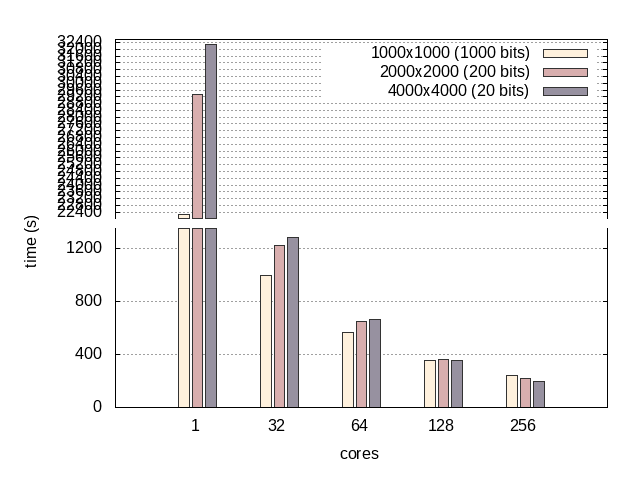
\includegraphics[width=\textwidth]{nodes_histogram}
      \end{center}
      \end{column}
      \begin{column} {.45\textwidth}
        \begin{center}
          \uncover<2->{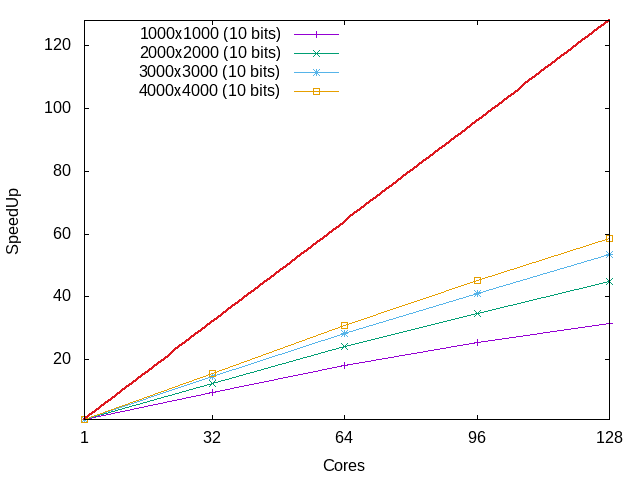
\includegraphics[width=\textwidth]{nodes_SPEEDUP}}
        \end{center}
      \end{column}
    \end{columns}
}
  \end{block}
\end{frame}
%%%%%%%%%%%%%%%%%%%%%%%%%%%%%%%%%%%%%%%%%%%%%%%%%%%%
\subsection{T5.4: Singular}
\begin{frame}
  \frametitle{T5.4 Singular}
  \begin{block}
    {D5.13: Paralel sparse polynomial multiplication}
  \end{block}
\end{frame}

%%%%%%%%%%%%%%%%%%%%%%%%%%%%%%%%%%%%%%%
\section{Workpackage management}

\subsection{Milestone M8}
\begin{frame}
  
\end{frame}
%%%%%%%%%%%%%%%%%%%%%%%%%%%%%%%%%%%%%%%%%%%%%%%%%
\subsection{Addressing remarks from previous review}
\begin{frame}
  
\end{frame}
%%%%%%%%%%%%%%%%%%%%%%%%%%%%%%%%%%%%%%%
%%%%%%%%%%%%%%%%%%%%%%%%%%%%%%%%%%%%%%%
\end{document}
